\chapter{Implementation}

Explain what you did to implement your solution, problems that occurred and how you fixed them. 
If they are interesting, include some relevant parts of the implementation (most relevant pieces of code and so on). 


\section{Program Structure}


each robot autonomously request task from the centralized pool and centralized pool response with a set of suitable tasks. 
\subsection{Robot Components}


\begin{figure}[htbp]
	\centering
	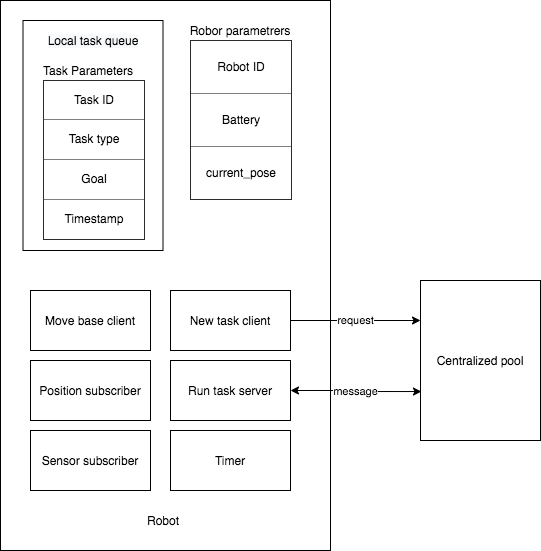
\includegraphics[width = 0.45\textwidth]{content/images/ch3/system_component_robot.drawio.png}
	\caption{Robot Components}
	\label{fig:robot_components}
\end{figure}

\begin{itemize}
	\item \textsl{Robot ID.} Robot ID is a unique identification for each robot.
	\item \textsl{Battery level.} Battery level drops as the robot moves and rotates.
	\item \textsl{Task type.} Robots perform different tasks such as "Charging", " Execute Task", "Gather Enviroment Information". For details please refer to Section \ref{sec:task_types}
	\item \textsl{Local task queue.} Local task queue keeps a list of tasks that a robot will run sequentially. Once a task is finished, it would be removed from task queue. Once this queue become empty, the robot send task result to centralized pool.
	\item \textsl{New task client.} Once all task are finished, the new task client send request to new task server.
	\item \textsl{Run task server.} The run task server receive tasks and send task feedback and task result.
	\item \textsl{Timer.} To prevent robot to be hanged by one task forever, the timer check the robot moving state periodically.
	\item \textsl{Move base client.} The move\_base node provides a ROS interface for configuring, running, and interacting with the navigation stack on a robot. The move\_base client send a goal to move\_base node to tracking their status  
	\item \textsl{Position subscriber.} The position subscriber get robot current position from navigation stack. The robot send its current location to centralized pool to request a new task.
	\item \textsl{Sensor subscriber.} The Sensor subscriber listen to sensor data within the range.
\end{itemize}

\subsection{Centralized Pool Components}

\begin{figure}[htbp]
	\centering
	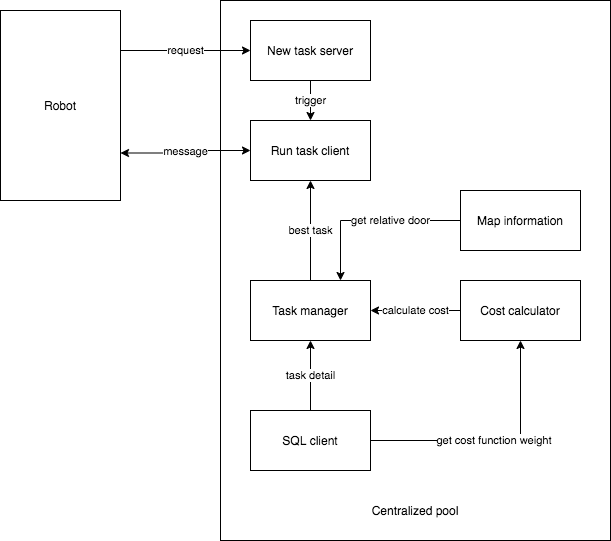
\includegraphics[width = 0.45\textwidth]{content/images/ch3/system_component_centralized_pool.drawio.png}
	\caption{Centralized Pool Components}
	\label{fig:centralized_pool_components}
\end{figure}

\begin{itemize}
	\item \textsl{Map Information.} Map information contains information such as the door list that the robot will pass through when moving to target position.
	\item \textsl{Cost calculator.} Cost calculator calculate the cost for doors, rooms and charging stations.
	\item \textsl{Task manager.} Task manager can construct, sort and allocate tasks.
\end{itemize}


\section{Communication Protocols}

\begin{figure}[htbp]
	\centering
	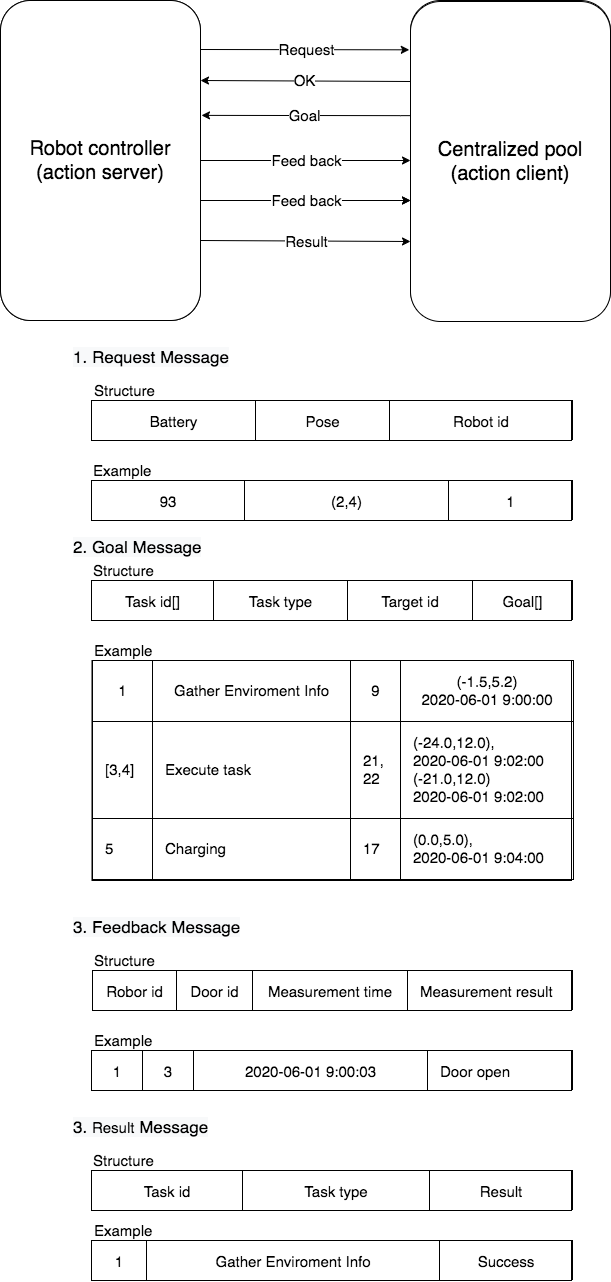
\includegraphics[width = 0.45\textwidth]{content/images/ch3/communication_protocals.drawio.png}
	\caption{Communication Protocols}
	\label{fig:communication_protocals}
\end{figure}

Since centralized pool and robots need to share task information with each other, the communication protocals are required. Four types of message are defined: (1) task request message; (2) task goal messages; (3) task feedback; (4) task result. 
The comparation of task type and examples of each type are shown in Figure \ref{fig:communication_protocals}. 

